\section{Application}
\label{sec:application}


\begin{figure*}[t!]
	\centering
	\begin{minipage}{.31\textwidth}
		\subfloat[Intra-server]{                    
			%\begin{minipage}{0.4\textwidth}
			\centering
			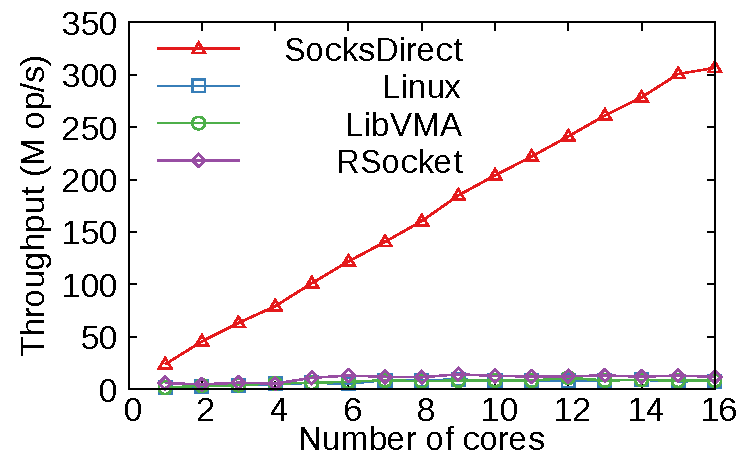
\includegraphics[width=\textwidth]{eval/microbenchmark/corenum-IPC-tput.pdf}
			\label{fig:eval-cornum-ipc}
			%\end{minipage}
		}
		
		\subfloat[Inter-server]{
			%\begin{minipage}{0.4\textwidth}
			\centering 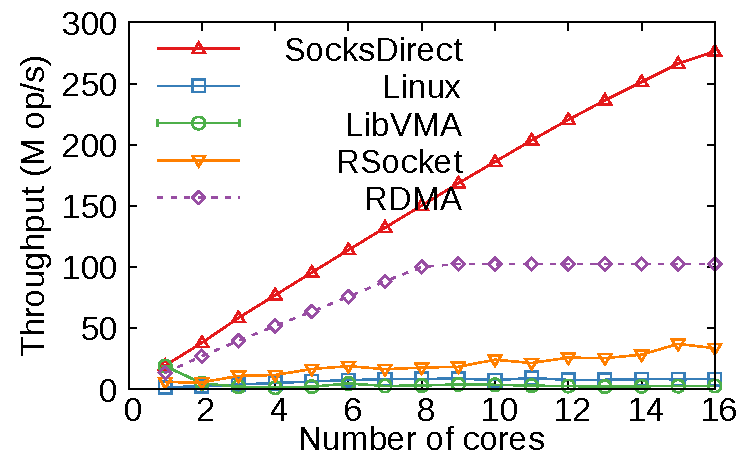
\includegraphics[width=\textwidth]{eval/microbenchmark/corenum-network-tput.pdf}
			\label{fig:eval-cornum-network}
			%\end{minipage}
		}
		\caption{Data transmission throughput with number of cores.}
		\label{fig:eval-corenum-tput}
	\end{minipage}
	\hspace{0.01\textwidth}
	\begin{minipage}{.31\textwidth}
		\centering
		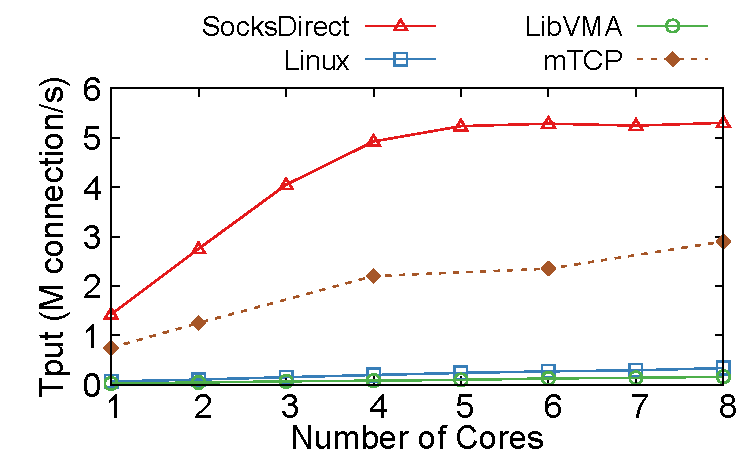
\includegraphics[width=\textwidth]{eval/microbenchmark/conn-setup-tput.pdf}
		\vspace{-10pt}
		\caption{Connection creation throughput with number of cores.}
		\label{fig:eval-conn-setup-tput}
		
		%\begin{minipage}{0.4\textwidth}
		\centering 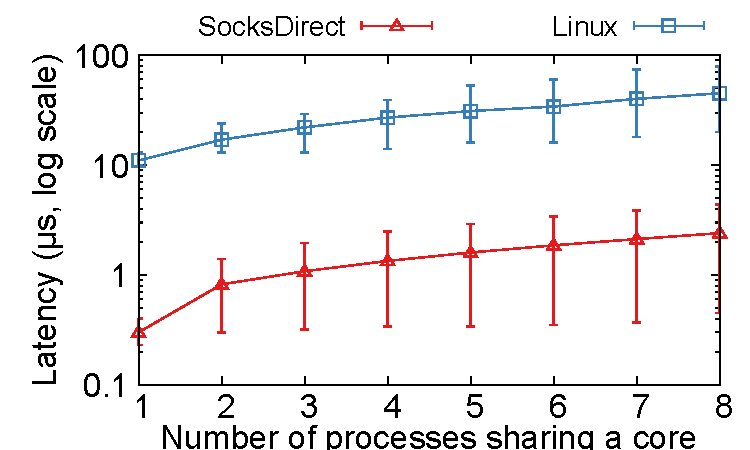
\includegraphics[width=\textwidth]{eval/microbenchmark/sharecore-lat.pdf}
		\vspace{-15pt}
		\label{fig:eval-context-switch}
		\caption{Latency of multiple processes sharing a core.}
		%\end{minipage}
	\end{minipage}
	\hspace{0.01\textwidth}
	\begin{minipage}{.31\textwidth}
		\centering
		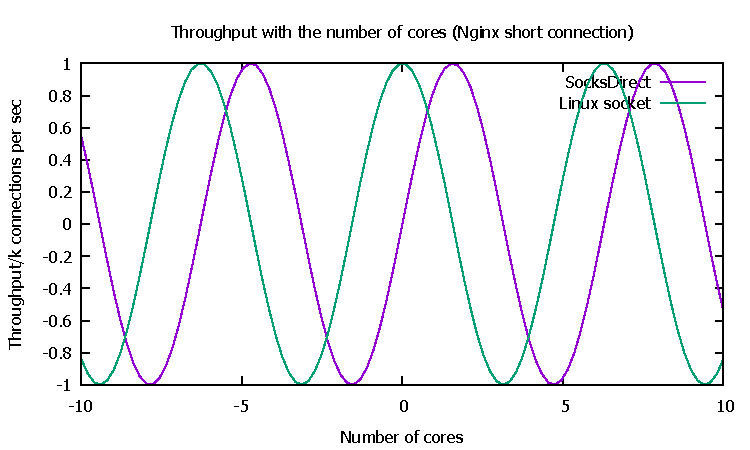
\includegraphics[width=\textwidth]{eval/microbenchmark/nginx-short-tput.pdf}
		\vspace{-15pt}
		\label{fig:eval-nginx-short}
		\caption{Nginx throughput.}
		
		\centering 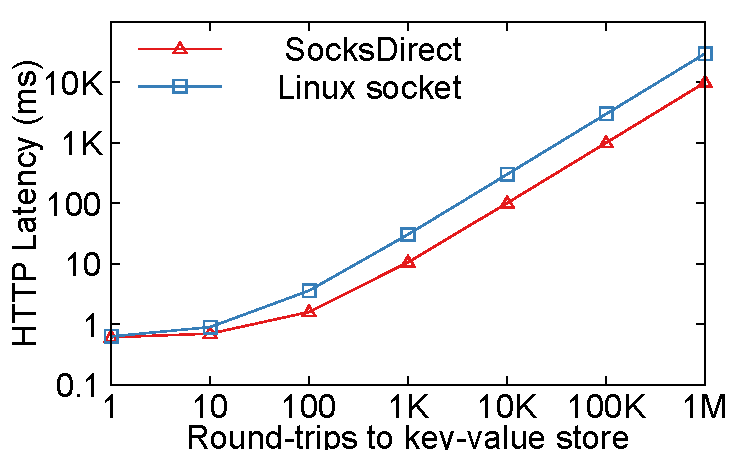
\includegraphics[width=\textwidth]{eval/microbenchmark/nginx-multiround-tput.pdf}
		\vspace{-15pt}
		\caption{HTTP request latency of a web service composed of Nginx, C++ application and memcached.}
		\label{fig:eval-nginx-multiround}
	\end{minipage}
\end{figure*}

\subsection{Network Function}

Network functions~\cite{li2016clicknp}, ClickOS~\cite{martins2014clickos}

Scenarios: Firewall (no packet change), NAT (change a packet field), Tunnel endpoint (add/remove packet header, change length)

Metrics: Latency, throughput

\begin{figure}[htpb]
	\centering
	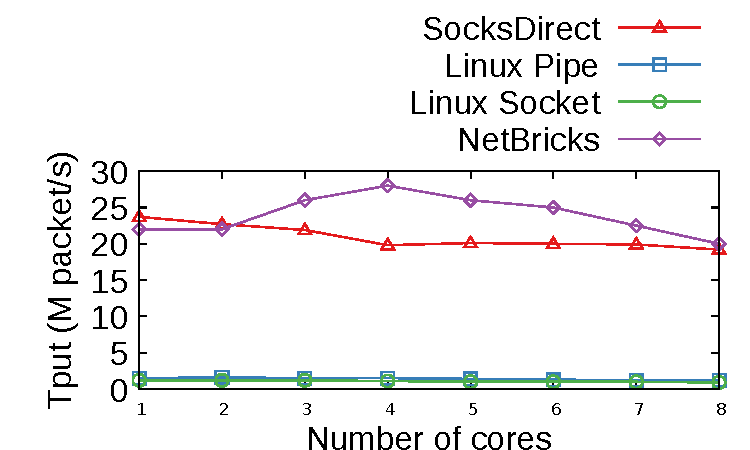
\includegraphics[width=0.33\textwidth]{eval/microbenchmark/nfv-tun-tput.pdf}
	\caption{Throughput of NFV tunnel}
	\label{fig:eval-tun-tput}
\end{figure}



\subsection{Web Application}

Nginx~\cite{nginx}, Nodejs~\cite{nodejs} and memcached~\cite{memcached}

\begin{itemize}
	\item Figure~\ref{fig:eval-nginx-short}: Many short-lived connections. Nginx $\rightarrow$ Nodejs, Nodejs access memcached once.
	\item Figure~\ref{fig:eval-nginx-multiround}: Each connection, backend interact extensively. (Nodejs access memcached multiple round trips.)
\end{itemize}


%\subsection{Real-time Stream Processing}

%Apache Flink~\cite{carbone2015apache} (need to turn off durability on disk)

%Scenario: Word Count (distributed system with one source, two mappers and one reducer)

%Metrics: Latency, throughput

%\subsection{Machine Learning}

%Tensorflow~\cite{abadi2016tensorflow}

%Scenario: (Distributed Tensorflow) Parameter server and worker on a same server.

%Metrics: Time per iteration